\documentclass {CSEThesis}
% Standard packages
\usepackage{amsmath}        % Extra math definitions
\usepackage{graphics}       % PostScript figures
\usepackage{setspace}       % 1.5 spacing
%\usepackage{psfig,epsfig}
\usepackage{multicol}
\usepackage{subfig}
\usepackage{epsfig,color}
% Custom packages
%\usepackage[first]{datestamp}   % Datestamp on first page of each chapter


\usepackage{color}
%===== page layout
% Define the side margins for a right-side page
%\insidemargin = 1.3in \outsidemargin = 0.9in
% Above margin is space above the header
% Below margin is space below footer
%\abovemargin = 1.5in \belowmargin = 0.05in


\btptitle = {Photonic Neuron for Artifical Neural Networks} % { and } are needed around your name
\name = {Student Name}          % and other feilds. don't remove.
\rollno = {03010104} \email = {id.iitp.ac.in} \guide = {Your guide
name}


\begin{document}

\begin{titlepage}
\begin{center}
\textheight 15.5in \textwidth 12.5in {\large\sf  \textbf{\the\btptitle}}\\[12ex]
{\small{\textsl{ \textbf{A B. Tech Project Report Submitted \\
in Partial Fulfillment of the Requirements \\
for the Degree of
\\[3ex]\small \bf Bachelor of Technology}}}}\\[16ex] \emph{by} \\[2ex]
{\sf \sf \textbf{\the\name}\\
             (\the\rollno)}\\[1ex]
\emph{under the guidance of}\\[2ex]
{\sf \bf \the\guide} \\[7ex]

\vspace{1in}

 \begin{figure}[!h]
 \hfill
 
\psfig{file=iitp_logo.eps,width=0.1\textwidth} \hfill \
 \end{figure}

{\sl \bf{to the}} \\[1ex]

{\small\bf DEPARTMENT OF ELECTRICAL ENGINEERING}  \\[1ex]
{\small \bf{INDIAN INSTITUTE OF TECHNOLOGY PATNA \\PATNA - 800013,
BIHAR}}
%\\[2ex]
%
%  {\color{red} \hrule height 0.5ex}
% \vskip 1ex
% May \the\year
\end{center}
\end{titlepage}

\cleardoublepage
\raggedbottom
\doublespacing
\pagenumbering{roman}
\chapter*{\centering \underline{CERTIFICATE}}
\vskip 2ex \emph{\quad This is to certify that the work contained
in this thesis entitled ``\textbf{\the\btptitle}'' is a bonafide
work of \textbf{\the\name} (\textbf{Roll No. \the\rollno}),
carried out in the Department of Computer Science and Engineering,
Indian Institute of Technology Patna under my supervision and that
it has not been submitted elsewhere for a degree.} \vskip 15ex
\begin{flushright}
Supervisor: \textbf{\the\guide}\\\end{flushright}
~~~~~~~~~~~~~~~~~~~~~~~~~~~~~~~~~~~~~~~~~~~~~~~~~~~~~~~~~~~~~~~~~~~~~~~~~~~~~
\hfill Assistant/Associate Professor,\\
May, \the\year~~~~
\hfill Department of Computer Science $\&$ Engineering,\\
Patna.\hfill Indian Institute of Technology Patna, Bihar.

\cleardoublepage
\chapter*{\centering Acknowledgements}
\quad{I would like to express my thanks to the Supervisor, Dr. Sumanta Gupta for non stop support throughout the project. A special thanks to all my colleagues who helped me in exchanging ideas, thoughts and made it possible to carry out the project with the accurate information. I thank my parents for their personal support and attention to inspire me. And finally God for making this all possible for me till the end.}
\cleardoublepage
\tableofcontents
\cleardoublepage
\addcontentsline{toc}{chapter}{List of Figures}
\listoffigures
\cleardoublepage
\addcontentsline{toc}{chapter}{List of Tables}
\listoftables
\cleardoublepage
\pagenumbering{arabic}
\def\headrulehook{\color{black}}      % Color the header rule

%========== Chapters
\typeout{}
\chapter{Introduction}
\pagenumbering{arabic}\hspace{3mm}

Ever since machine learning has been introduced into the field of computer science, it has been spearheading breakthroughs in a number of fields. It has taken the world by storm and now, many fields will simply cease to function without these techniques. Deep learning is one sub-field of machine learning which is deeply rooted in todays society. Deep learning is now part of common man's everyday life and it will remain so for the forseeable future.

As data collection and storage becomes more prominent, machine and deep learning has continued to dominate the data space, provide insights into complex data which is simply not possible with other mathematical methods. Deep learning is one of the most rapidly expanding machine learning technologies, relying on multi-layered artificial neural networks (ANNs) implemented in digital electronics to handle big data sets, integrating and analysing massive volumes of information quickly without the need for explicit instructions. These ANNs have been modified and augmented in many ways, leading many domain specific techniques, most notable one being Convolutional Neural Networks (CNNs) which is primarily used in image analysis.

\section{Artifical Neural Networks}

Artificial neural networks refers to those algorithms which are inspired by the biological neural networks that constitute animal brains. Such systems learn to perform tasks by considering examples, generally without being programmed with any task-specific rules. For example, in image recognition, they might learn to identify images that contain cats by analyzing example images that have been manually labeled as "cat" or "no cat" and using the results to identify cats in other images. They have found most use in applications difficult to express with a traditional computer algorithm using rule-based programming.

Traditionally ANNs have been described as a black box of sorts. It has a number of input variables and output variables using simple arithmetic connections, gives output from the input.

\begin{figure}
	\centering
	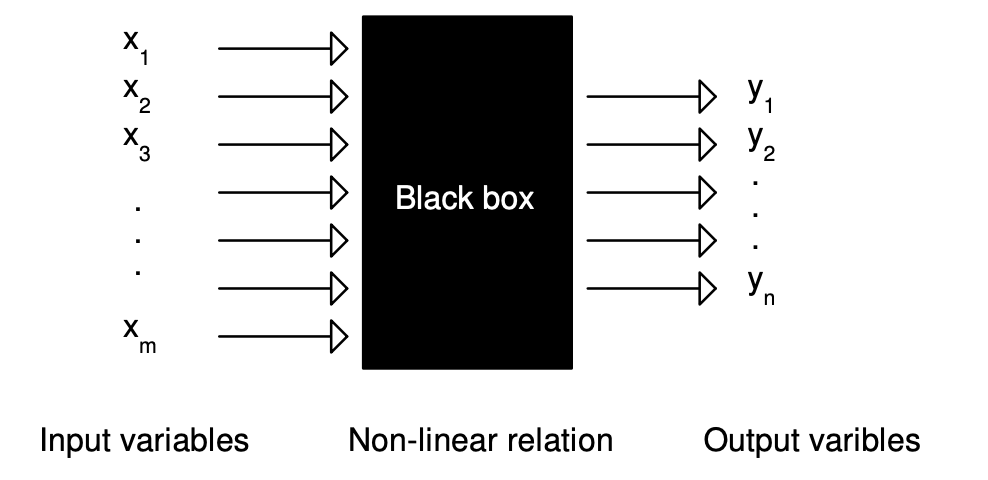
\includegraphics[width=0.5\textwidth]{images/ann.png}
	\caption{Blackbox representation of a ANN}
	\label{fig:neuron}
\end{figure}

ANNs Traditionally tend to excel where the relations between inputs and outputs are non-linear. It is practically better and more efficient at classifying or identifying non-linear relationships rather that linear ones, where it might perform worse than a more statistical approach.

Nowadays, the most common type of ANN is the feedforward neural network, which consists of a group of neurons (called a layer) that transfer data to another group of neurons in a feedforward manner. The first layer is called the input layer, and the last layer is called the output layer. The layers in between are called hidden layers. The input data travels through the layers in a feedforward manner, and the output is the result of the last layer. The output is then compared to the expected output, and the error is calculated. The error is then backpropagated through the network, and the weights are adjusted accordingly. This process is repeated until the error is below a certain threshold.

\begin{figure}[h]
	\centering
	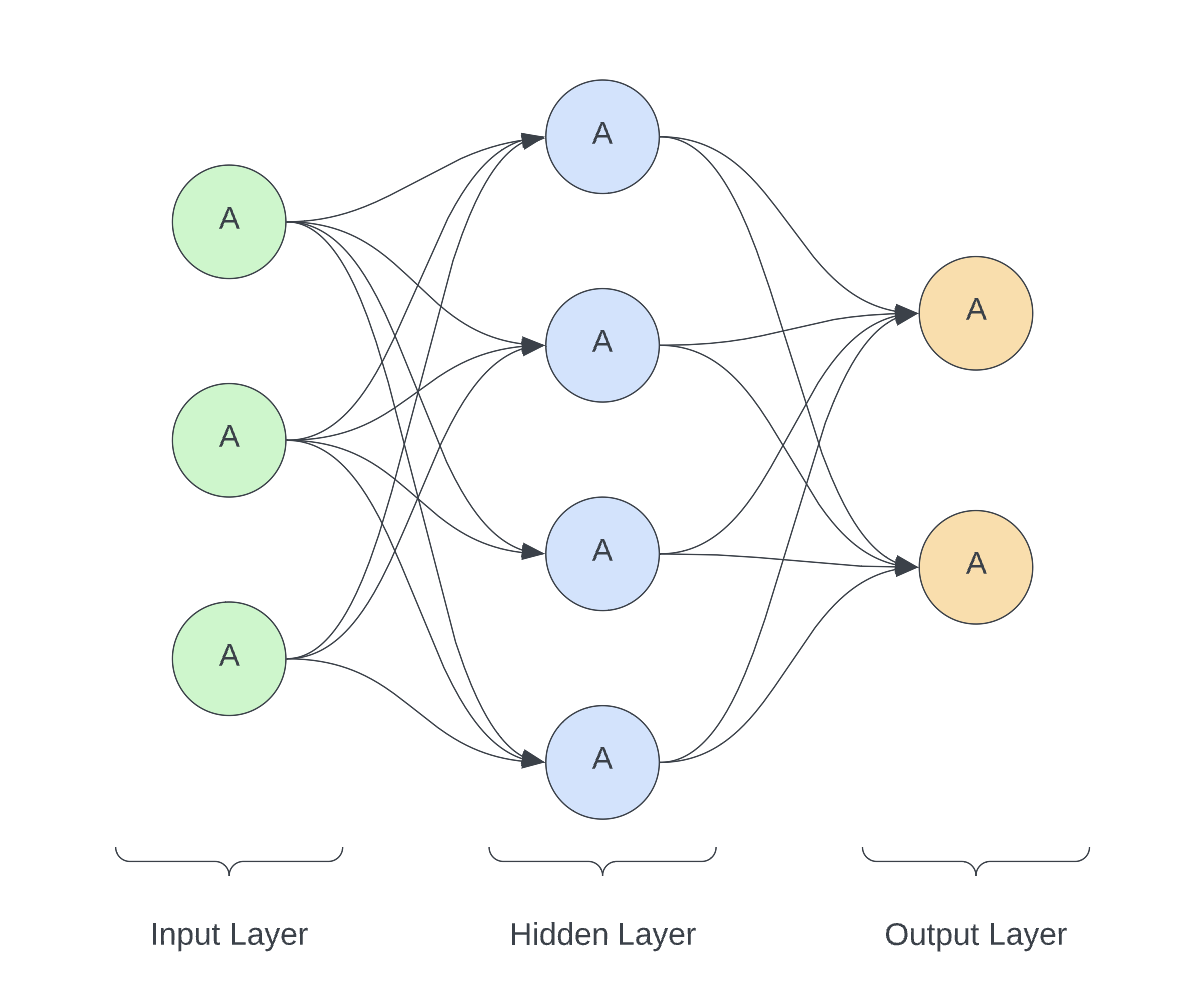
\includegraphics[width=0.7\textwidth]{images/feedforwardANN.png}
	\caption{Feedforward ANN}
\end{figure}

\section{Convolutional Neural Networks}

Convolutional Neural Networks (CNNs) are a class of deep neural networks, most commonly applied to analyzing visual imagery. They are also known as shift invariant or space invariant artificial neural networks (SIANN), based on their shared-weights architecture and translation invariance characteristics. They have applications in image and video recognition, recommender systems, image classification, medical image analysis, natural language processing, brain-computer interfaces, and financial time series.

CNNs usually apply convolution operation over the image (hence the name) by using a filter, called the kernel. This produces a smaller image but where features can be extracted easily. Diiferent filters are applied to the same image in the form of multiple channels resulting in diverging features in each channel which can be detected. This is called feature mapping. The feature maps are then flattened and fed into a fully connected ANN which gives the final output. The application of kernel is illustrated in figure \ref{cnn}.
\\
\begin{figure}[h]
	\centering
	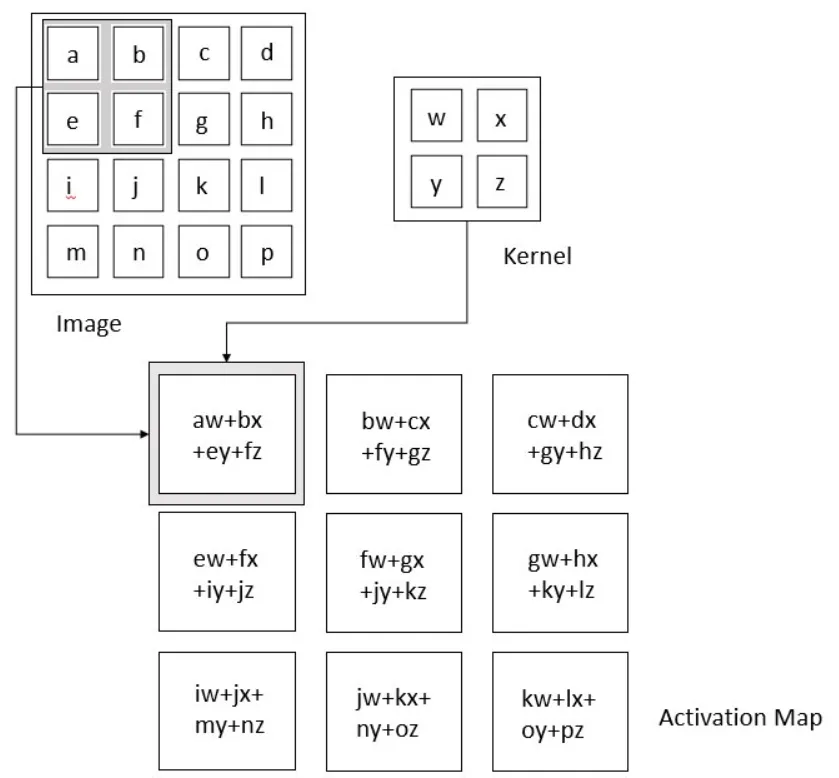
\includegraphics[width=0.8\textwidth]{images/cnn.png}
	\caption{Working of kernel and convolution in CNNs \cite{Goodfellow-et-al-2016}}
	\label{cnn}
\end{figure}

\section{Conventional Implementation of Neural Networks}

Neural networks, for the most part, have been software based. The algorithms are implemented in code and is executed in high-power GPUs for fast parallel computations. This form is extremely flexible and can be used for a variety of applications. The model can be changed as and when the need arises and is reletively commitment-less. The hardware itself is also largely independent of the software and changed/replaced whenever deemed necessary.

There has been a recent growth in certain of Application Specific Integrated Circuits (ASICs) specifically for neural networks, some notable examples being from popular manufactors like NVIDIA \cite{NVIDIAT4Tensor} and Apple. These chips are designed to perform neural network computations and are extremely fast and efficient. They are also extremely expensive and are not easily available.

Even with the advent of ASICs in Machine learning space, the field still suffers from the fact that the hardware is not really coupled with the software. By increasing the specificity of the hardware, the efficiency of the system can be increased by a large margin.

\section{Disadvantages of Conventional Implementation}

The conventional implementation of neural networks has a number of disadvantages. The most prominent one being the fact that the hardware is not really coupled with the software. The hardware is not really designed to perform neural network computations and is not really efficient at it. Large amounts of power are required to train models for prolonged amounts of time. This leads to a lot of inefficiencies in the system.

\section{Photonic Neuron}

As discussed, the conventional implementation of neural networks has a number of disadvantages. The hardware is not really designed to perform neural network computations and is not really efficient at it. This sparks the question "What can be a proper hardware implementation of neuron, the basic structure of a neural network, that can be used to perform neural network computations efficiently?". The answer to this question that this thesis proposes is the Photonic Neuron.

The photonic neuron exploits the fact that multiplication can be done essentially for free in the photonics domain through the use fo hardware like Mach-Zehnder Interferometers or Micro-Ring Resonators. Photonics is known to be inherently very fast since most of the operations are done in speeds close to the speed of light. This makes it a very good candidate for the speed up of existing hardware implementation.

Many prospective applications become blaringly obvious when we consider the speeds that photonics really has to offer. When we also consider the power efficiency of such a implementation, we can see the possibilities. Easily identifiable applications include on-device deployments of trained models for applications like self-driving cars, drones, etc. These require highly power efficient and latentcy-less neural network implementation which photonics can offer.

\section{Diiferent Architectures of Photonic Neurons}

There are a number of different architectures of photonic neurons that have been proposed. Some of them are discussed below.

One possible implementation is cascading a number of Mach-Zehnder Interferometers (MZIs) to perform the multiplication operation \cite{8961101}. MZIs can be efficiently used to achieve multiplication. Thus a series of MZIs can be cascaded as per the requirement of the model the achieve an efficient implementation of the neural network.

\begin{figure}
	\centering
	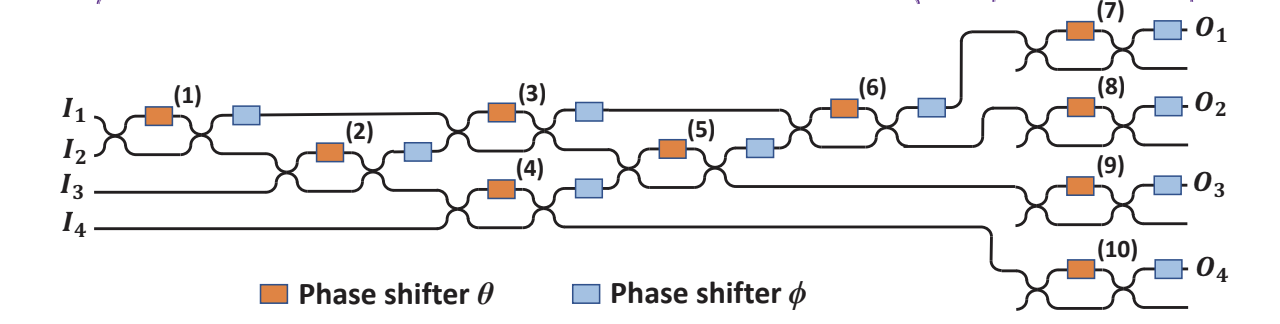
\includegraphics[scale=0.7]{images/cascadedMZI.png}
	\caption{Schematic diagram of a 4x4 MZI based photonic neuron}
	\label{4x4mzi}
\end{figure}

As is evident from the picture, the hardware complexity grows exponentially as the number of parameters increase, which is not really practical as the number of parameters in a neural network is usually very large, even reaching billions at times \cite{chowdhery2022palm}. This makes the implementation of such a system very difficult.

Another approach to making neural networks in photonics domain is using MicroRing Resonators (MRRs). This uses multiple MRRs in a cascaded fashion to implement a complete spiking neural network \cite{photonics9020120}. Although cascading MRR is somewhat better than cascading MZIs, it still suffers from the same problem of exponential growth of hardware complexity.

\begin{figure}
	\centering
	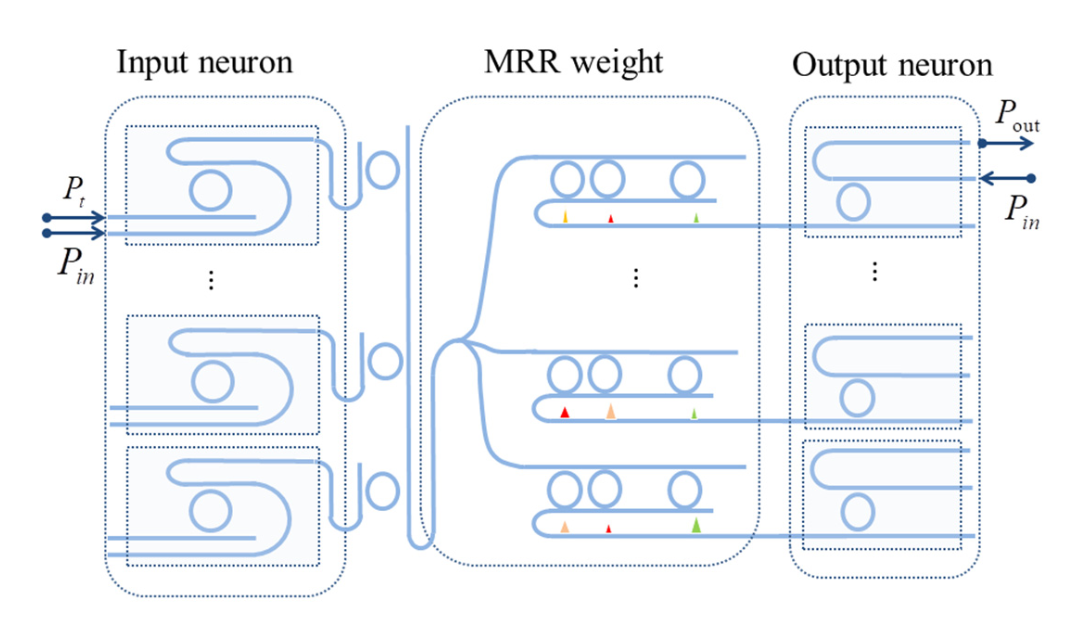
\includegraphics[scale=0.7]{images/cascadedMRR.png}
	\caption{Schematic diagram of a all MRR photonic neuron \cite{photonics9020120}}
\end{figure}

One way to overcome this issue is to use one resuable component for the repetitive operations of the neural network. Just like how GPU were employed for neural net calculations because they were efficient at parallel and repeptetive operations, we can use a small reusable neuron and reuse for the entire neural network.

Following in this path, the structure known as PEMAN was introduced \cite{demarinisCodesignedIntegratedPhotonic2022}. PEMAN stands for Photonic Electronic Multipication Accumulation Neuron. It proposes a hybrid photonic electronic neuron that can be reused many times to implement a complete neural network. The structure of PEMAN is shown in figure \ref{peman}.

\begin{figure}
	\centering
	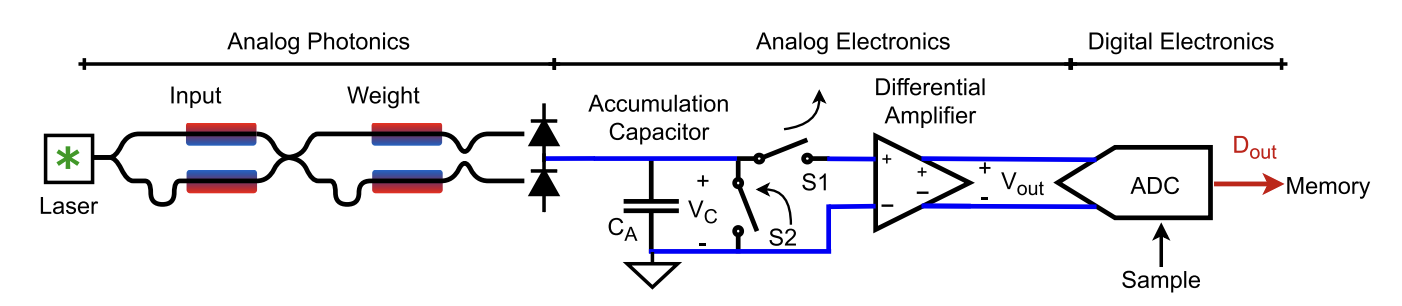
\includegraphics[width=\textwidth]{images/peman.png}
	\caption{Schematic diagram of a PEMAN \cite{demarinisCodesignedIntegratedPhotonic2022}}
	\label{peman}
\end{figure}

\section{Motivation}

The motivation behind this thesis is to explore the possibility of using a PEMAN like structure to implement a complete neural network. The PEMAN structure is a very good candidate for the implementation of a neural network in the photonic domain. It is highly reusable and can be used to implement a complete neural network. The PEMAN structure is also highly power efficient and can be used to implement a neural network that is highly power efficient.

In particular, this thesis aims to explore the creation of a artifical neural network and convolutional neural network architecture using the PEMAN structure. It also tries to explore the process of training on the said hardware implementation and study the accuracy, ENOB and time efficiency of the system.


\cleardoublepage
\typeout{}
\chapter{The PEMAN Structure}

The PEMAN structure is a hybrid photonic electronic structure which uses photonic operation for multiplication and electronic hardware for accumulation. It also has inbuilt non-linearity with the use of an ADC.

\section{Working Principle}

The PEMAN structure consists of three distinct sections: the analog photonics section, analog electronics section and digital electronic ssection. Each section applies one part of the ANN algorithm and is thus resuable inside a neural network. Each of the section is discussed in detail in the upcoming sections.

\subsection{Analog Photonics Section}

The analog photonics section is responsible for the multiplication of the input vector with the weight matrix. The multiplication of inputs and weights have been identified as the most computationally intensive part of the ANN algorithm and thus we can exploit photonics to the maximum extent by using it in this context.

In order to study how the multiplication works, a single MZI is first studied. Figure \ref{1x1mzi} shows the structure of an MZI.

\begin{figure}
	\centering
	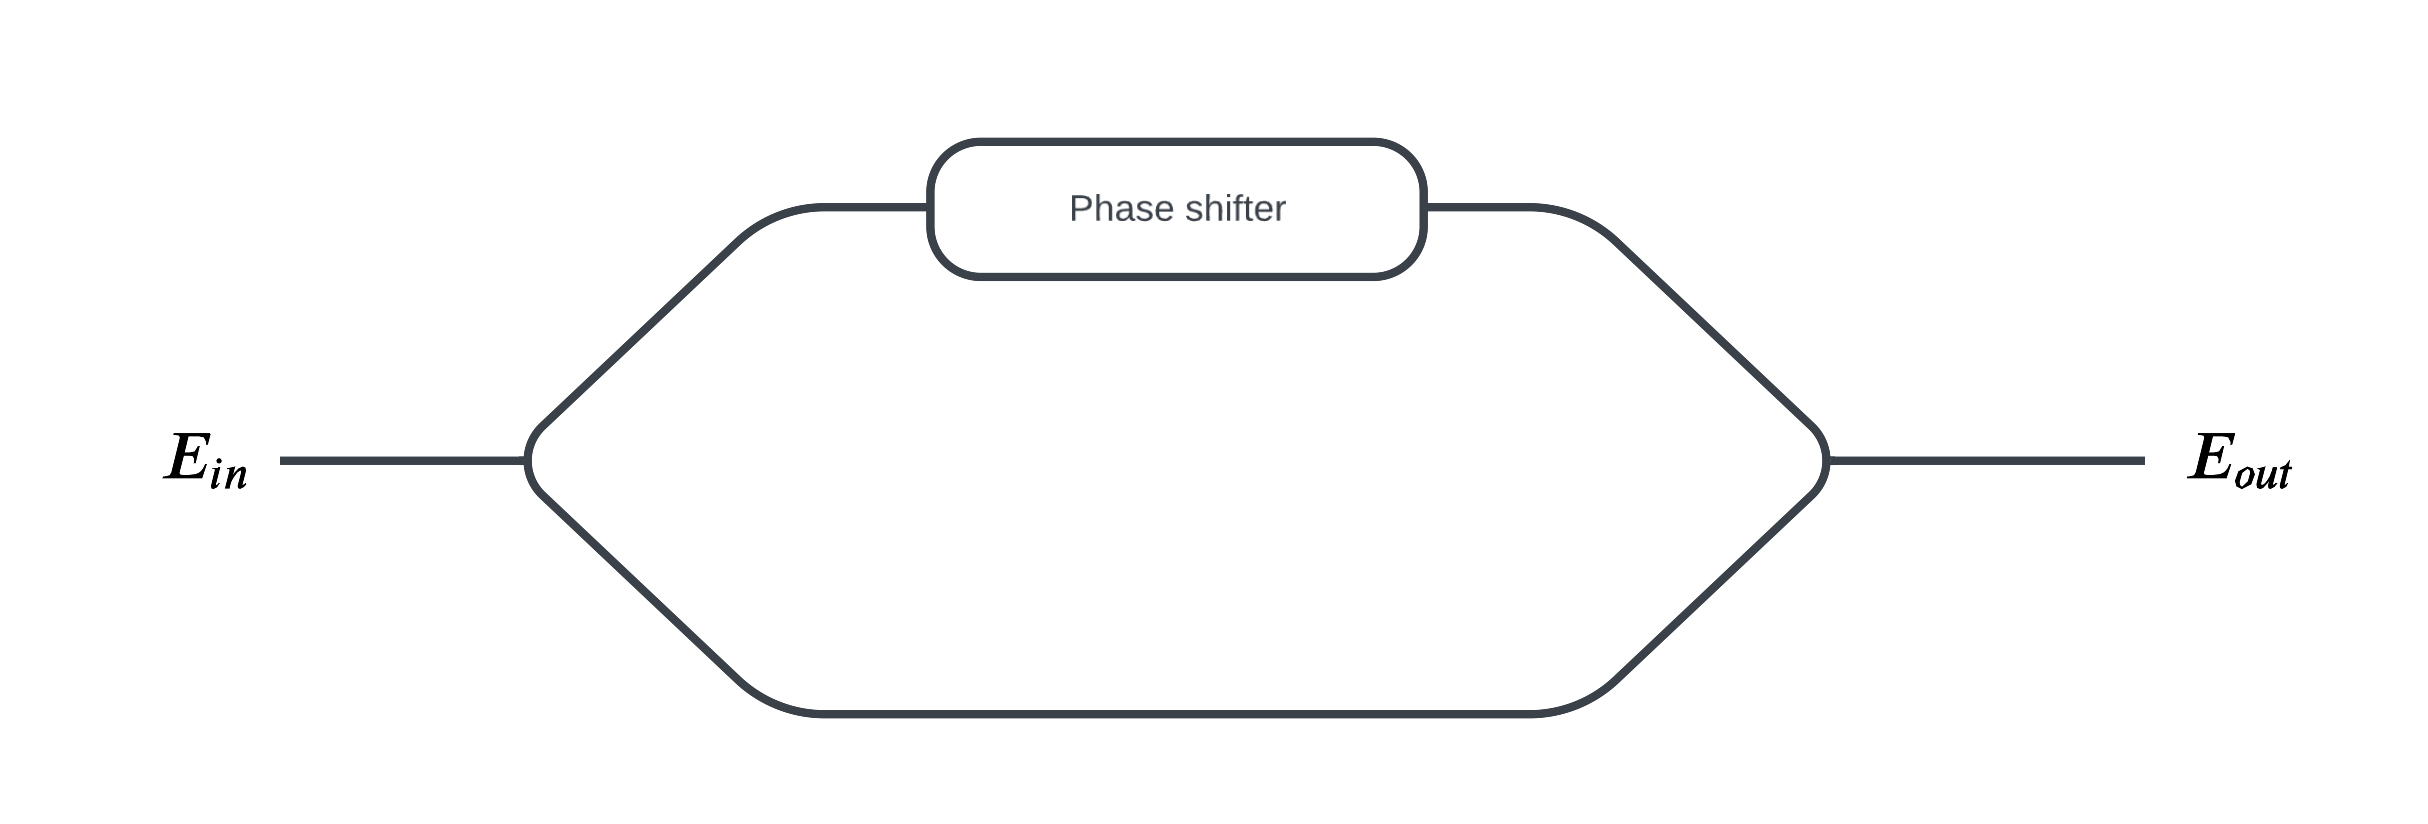
\includegraphics[width=\textwidth]{images/mzi.png}
	\caption{Schematic diagram of a 1x1 MZI}
	\label{1x1mzi}
\end{figure}

The structure is made up oftwo Y junctions on both sides with a phase shifter in-between. Lets say the input field is $E_{in}$, output field is $E_{out}$ and the phase shifter has a shift of is $\phi$. After applying the transfer matrices for each of the components, we get

\begin{equation}
	E_{out} = E_{in}\cos \phi
\end{equation}

This result can be interpreted as the multiplication of the input field with a value of $\cos \phi$. In PEMAN, the laser is generally given a constant current as it is reused for many operations. This means that the phase shifter needs to be changed dynamically to achieve multiplication.

In the actual PEMAN structure, two MZIs are used, one for input setting and one for weight setting, thereby giving the effect of multiplication of input and weight together.

Figure \ref{propPEMAN} depicts the structure that is used in this thesis as the PEMAN structure.

\begin{figure}
	\centering
	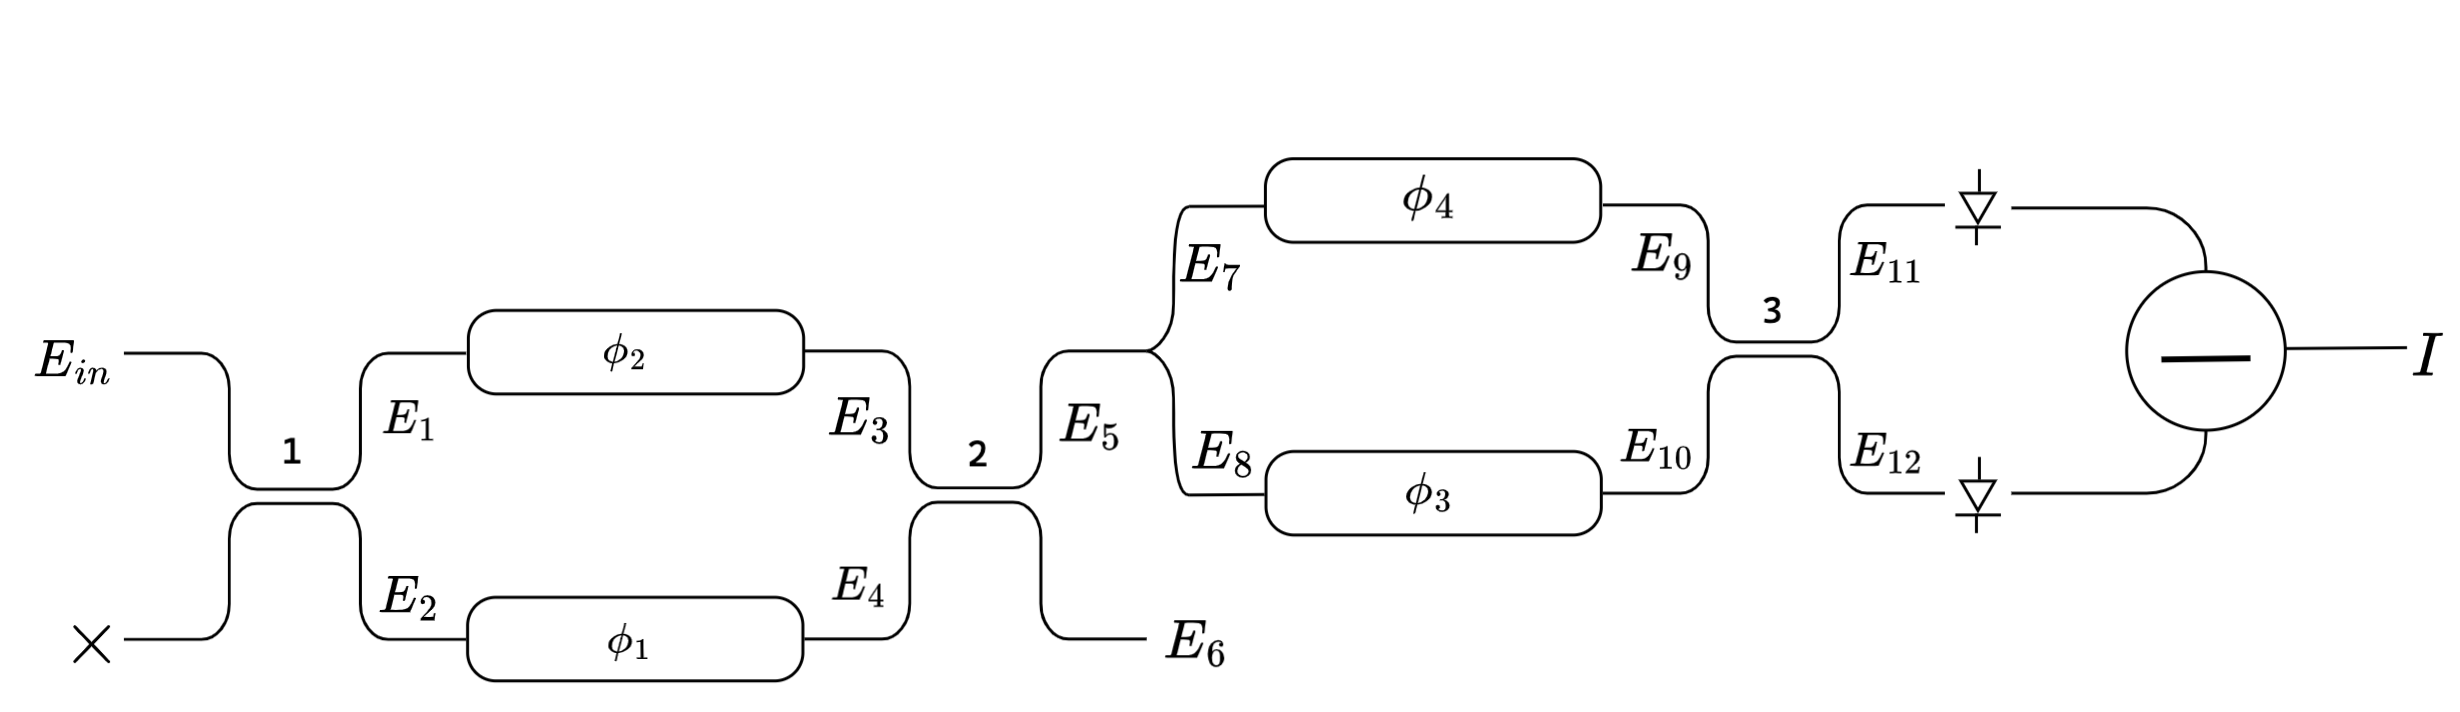
\includegraphics[width=\textwidth]{images/propPEMAN.png}
	\caption{Schematic diagram of the PEMAN structure}
	\label{propPEMAN}
\end{figure}

\subsection{Analog Electronics Section}

The analog electronics domain consists of a capacitor and a differential amplifier. These two components together is used as an accumulator to achieve the addition part in a neuron. Once the capacitor stores all the output produced by the photonics part, it is discharged into the next stage.

\subsection{Digital Electronics Section}

The digital electronics section consists of an ADC. This ADC is responsible to convert the analog current coming from the capacitor to digital domain. WHile converting, it is also implemented to apply a non- linear function to account for the activation function in a neuron. The ADC is also responsible for quantizing the output to a certain number of bits. Quantizing the values reduces the accuracy but boosts the overall speed.

\section{Timing Diagram}

Figure \ref{timing} shows the timing diagram of the PEMAN structure. The timing diagram shows the working of the PEMAN structure for a single neuron. It is necessary to study the time complexities and the under-workkings of the PEMAN structure in order to properly utilize its advantages.

\begin{figure}
	\centering
	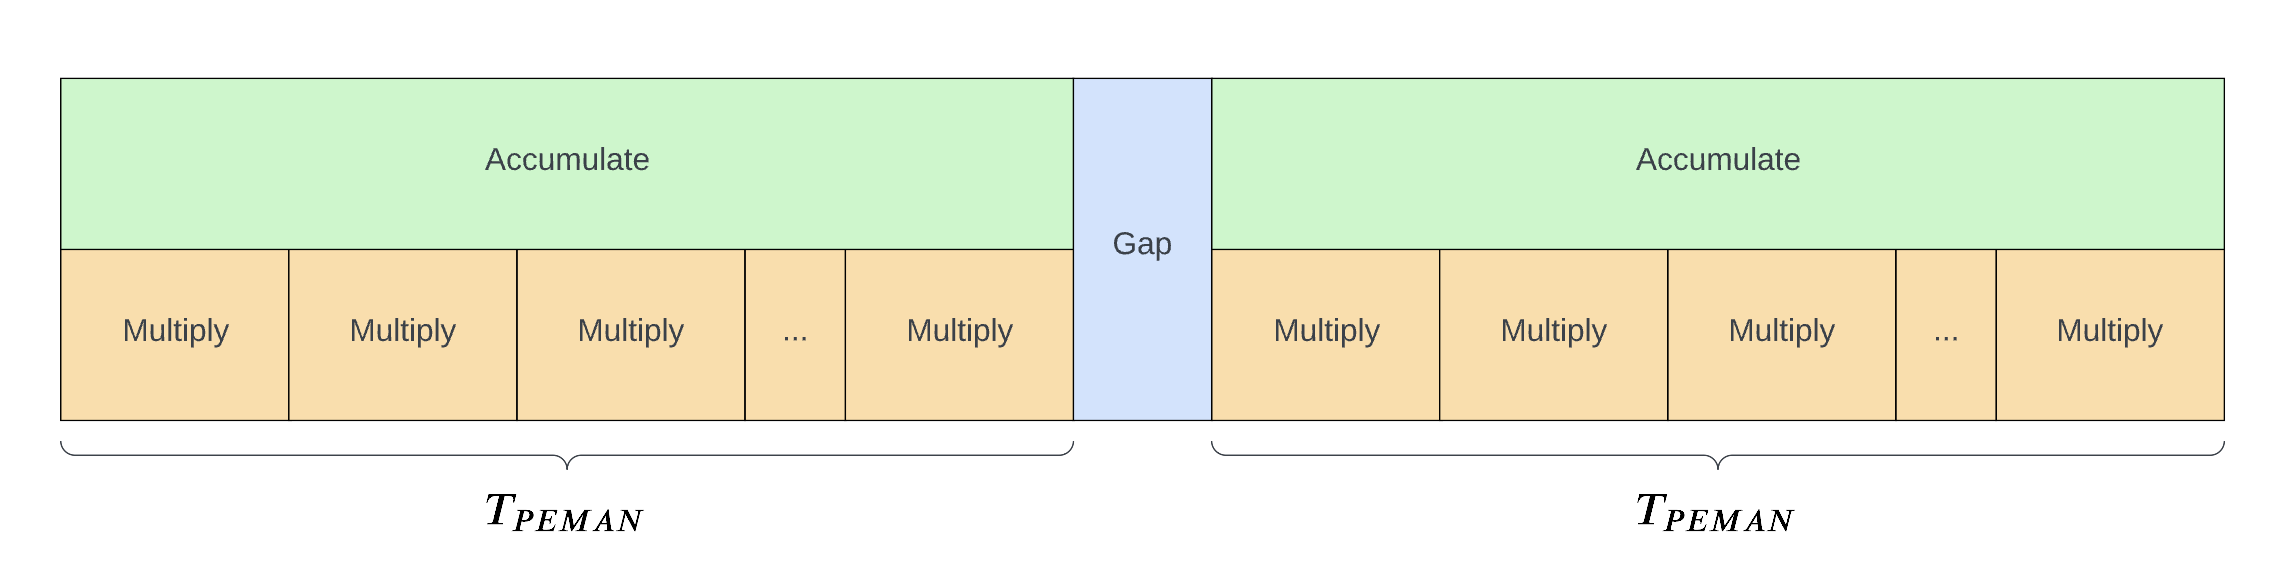
\includegraphics[width=\textwidth]{images/timing.png}
	\caption{Timing diagram of the PEMAN structure}
	\label{timing}
\end{figure}

From the figure, we can see that accumulation and the consecutive functions do not need to be as fast as multiplication. This is because multiplication is done a number of times before it has to be accumulated. This can also be leveraged by the fact that multiplication is done in the photonics domain and accumulation is done in the analog domain. This means that the multiplication can be done relatively fast while the accumulation can be done at a much slower speed.

\section{PEMAN Structure and Neural Networks}

The PEMAN structure is made to be reused such that an entire neural network can be implemented using the same structure. While it is implemented for the entire structure, we also need to consider training and inference.

\subsection{Conventional Method}

The conventional method to use a neural network built with the PEMAN structure involves using a GPU to train the model as normally done. Once the model has been trained to a satisfactory state, the weights are extracted. These weights are then matched with a premade lookup table to extract the necessary phase shifts for the weights. Now, when actual input is sent for inference, the inputs are converted to phases using the same lookup table, and set. The corresponding weight phases are set simultaneously. The output is then passed through the remainder of the structure and the final output is obtained.

This method is the traditional way to use PEMAN as we do not have to deal with reduced bit operation during training and can use effective quantization techniques to quantized the extract the weights without much drop in accuracy.

\subsection{Training on PEMAN}

Training on PEMAN is a relatively new concept. The idea is to train the model directly on the PEMAN structure. This means that the weights are not extracted from a GPU but are instead trained on the PEMAN structure itself. This is done by essentially using the same feedforward and backpropogation methods which are slightly modified to adapt to the new structure.

This approach can provide a significant speed boost to both training and inference as the weights do not need to be extracted and the entire model can be trained on the PEMAN structure itself. This also means that the model can be trained with reduced bit operation and thus can be trained faster. However, this approach is still in its infancy and needs to be studied in detail to understand its advantages and disadvantages.

One disadvantage might be that the reduced bit operation might degrade the accuracy more that necessary. But, upon testing for the handwritten digit recognition problem, it was found that the accuracy drop was not significant. This means that the reduced bit operation can be used to train the model faster without much drop in accuracy.

\section{Algorithm for training on PEMAN}

The process of training on PEMAN directly is fairly straightforward and bears a lot of resemblance to the original algorithm. The only real change is most of the operations now have an additional lookup step, which is necessary to convert the digital data to values of physical significance.

Figure \ref{trainOnPemanAlgo} shows the algorithm for training on PEMAN. The algorithm is divided into two parts: the feedforward part and the backpropogation part. The feedforward part is responsible for calculating the output of the network for a given input. The backpropogation part is responsible for calculating the gradients of the weights and biases and updating them.

\begin{figure}
	\centering
	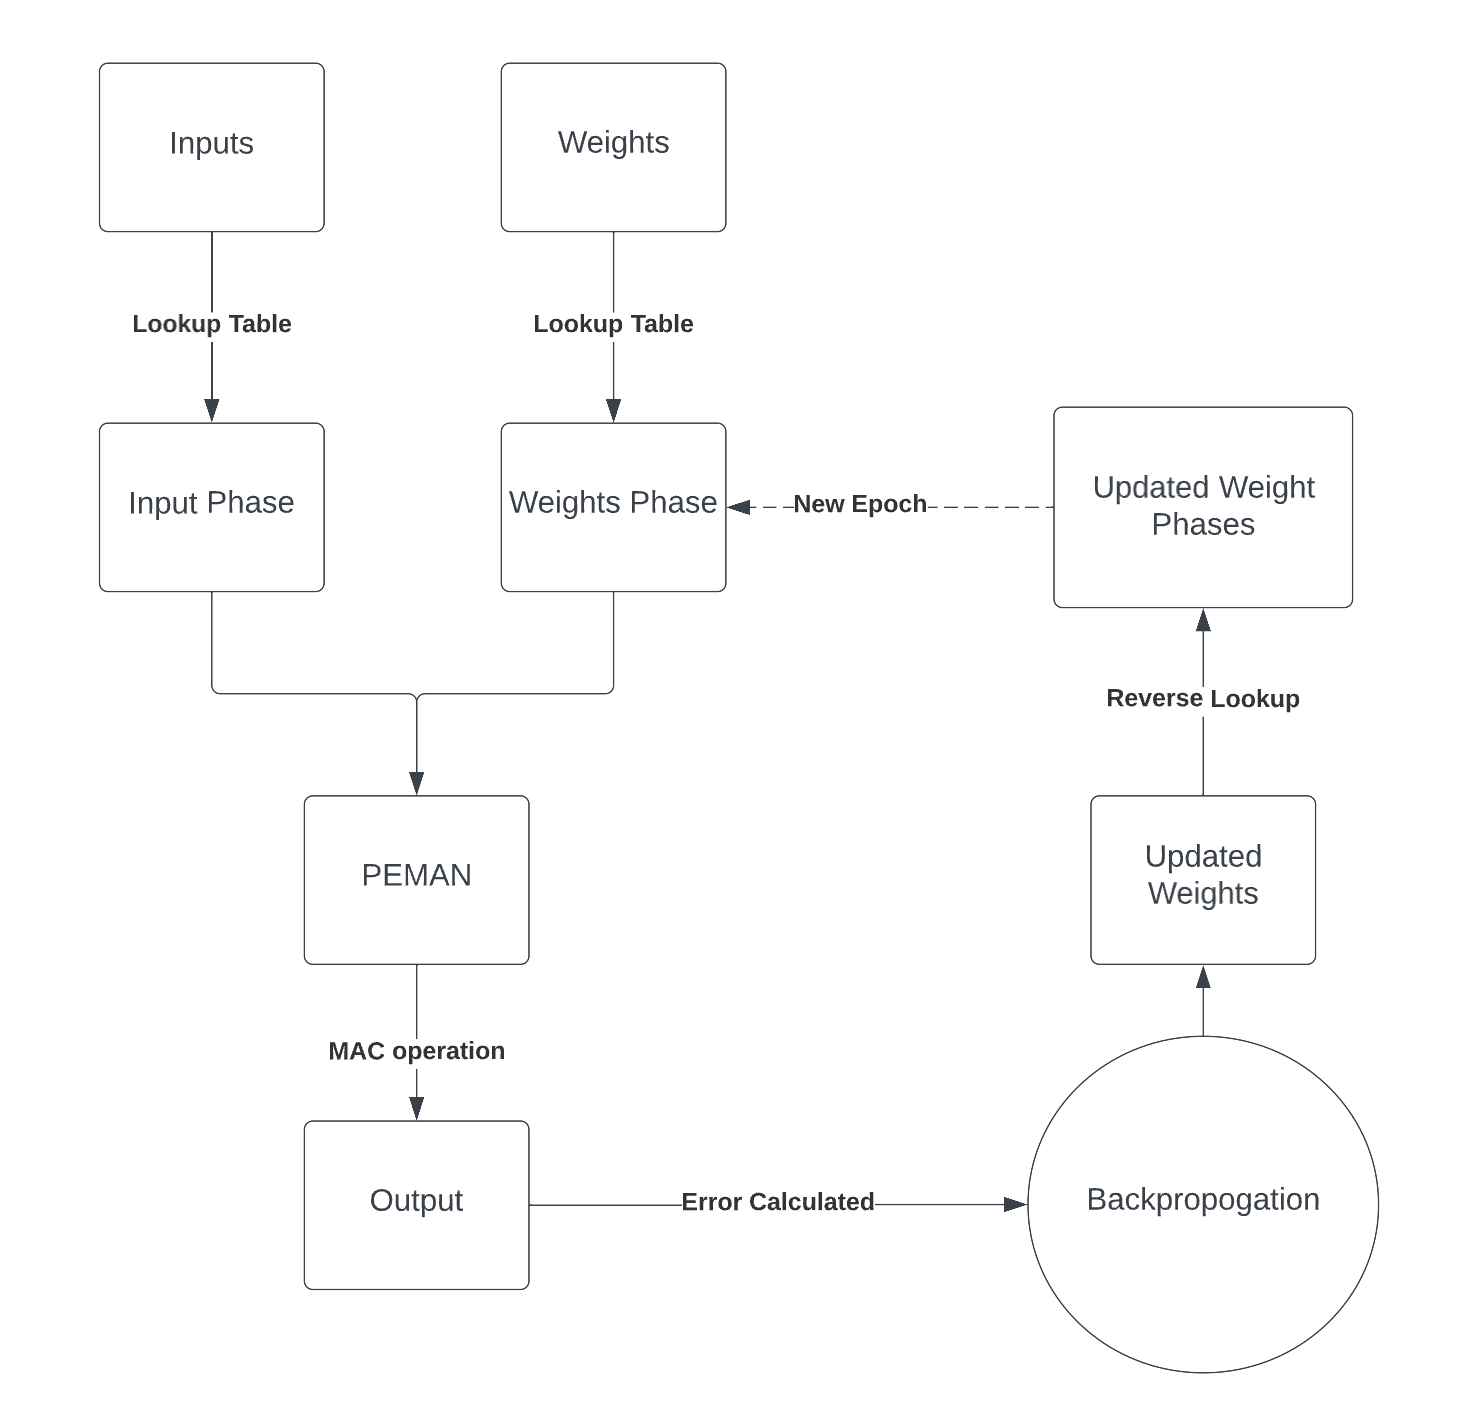
\includegraphics[width=\textwidth]{images/trainOnPemanAlgo.png}
	\caption{Algorithm for training on PEMAN}
	\label{trainOnPemanAlgo}
\end{figure}

Through using this technique, we employ the same backpropogation technique that has been proven to be successful while also modiying it so that we can train the phases of the PEMAN directly. This means that we can train the model directly on the PEMAN structure and thus can achieve a significant speed boost.

\section{PEMAN Structure and Handwritten Digit Recognition}

In order the study the practical implications of using such an approach, the handwritten digit recognition problem is used. The handwritten digit recognition problem is a classification problem where the goal is to classify a given handwritten digit into one of the 10 classes. The dataset used for this problem is the MNIST dataset. The MNIST dataset consists of 60,000 training images and 10,000 testing images. The images are grayscale images of size 28x28. The dataset is split into training and testing sets with a ratio of 6:1.

The model used for this problem is a simple feedforward neural network with 1 hidden layer. The input layer has $28 \cdot 28 = 784$ parameters. The hidden layer has 100 parameters. The output layer has 10 parameters. The activation function used is the ReLU function. The loss function used is the cross entropy loss function. The optimizer used is the Adam optimizer. The model is trained for 10 epochs with a batch size of 64.

The model was trained in the same architecture but two different times. The first time, post training quantization technique was applied to quantize the wieghts to 8 bits and then the inference was run. In the second case, all the inputs and weights were quantized to various bit resolution while training itself. This helps us simulate the difference between training on PEMAN versus only inference through PEMAN.

The model when only done post-training quantization achieved an accuracy of 98.10\%. Figure \ref{trainingOnPeman} shows the accuracy values achieved by the same model when trained with pre-quantized parameters.

\begin{figure}
	\centering
	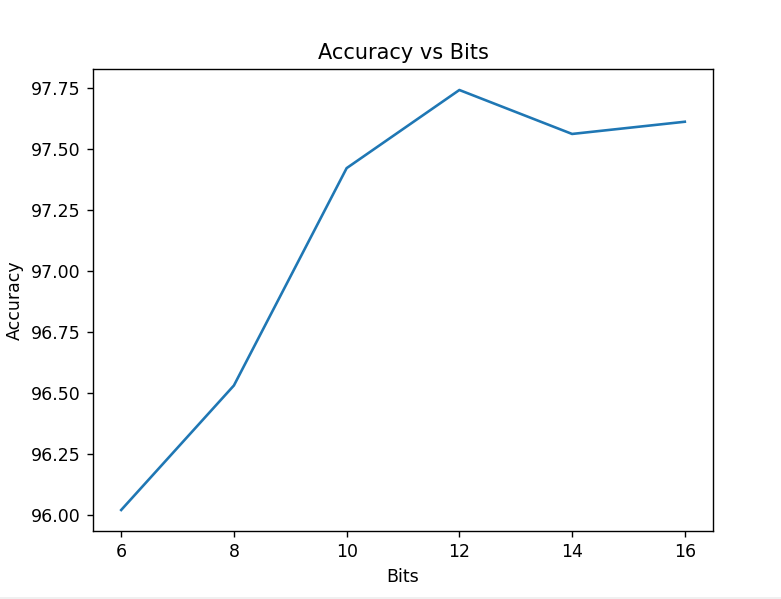
\includegraphics[width=\textwidth]{images/trainingOnPeman.png}
	\caption{Accuracy values achieved by the model when trained with pre-quantized parameters}
	\label{trainingOnPeman}
\end{figure}

From this plot, we can infer that at 8 bit resolution, we have an approximate accuracy of 96.50 \%, which is lower that 98.10\% achieved by the post-training quantization technique. However, we can also see that the accuracy is still quite high and the drop is not significant. This means that we can train the model with reduced bit operation and still achieve a high accuracy. This also means that we can train the model faster as the reduced bit operation is faster than the full bit operation.


\cleardoublepage
\typeout{}
\chapter{CNN Architecture}

Convolutional Neural Networks (CNNs) are a special kind of multi-layer neural networks. Like almost every other neural networks they are trained with a version of the back-propagation algorithm. Where they differ is in the architecture. CNNs are designed to recognize visual patterns directly from pixel images with minimal preprocessing. They can recognize patterns with extreme variability (such as handwritten characters), and with robustness to distortions and simple geometric transformations. They are also known as shift invariant or space invariant artificial neural networks (SIANN), based on their shared-weights architecture and translation invariance characteristics.

\section{Principle}

CNNs for the most part, work by taking an input image and apply convolution operations over it with a kernel. The weights of the kernel is continuously updated over the period of training using back-propogation.

\begin{figure}
	\centering
	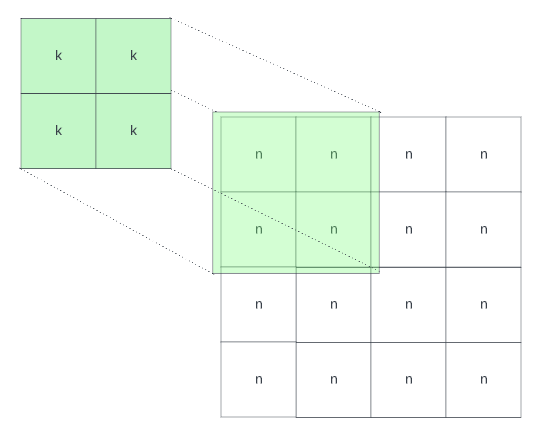
\includegraphics[width=0.5\textwidth]{images/convolution.png}
	\caption{Convolution operation}
	\label{convolution}
\end{figure}

Figure \ref{convolution} shows the convolution operation. The kernel is a matrix of weights which is applied over the input image. The kernel is slided over the image and the dot product of the kernel and the image is taken. The result of the dot product is stored in the output matrix. The kernel is slided over the image by a stride. The stride is the number of pixels by which the kernel is slided over the image. The kernel is slided over the image in both the horizontal and vertical direction. The output matrix is called the feature map. The feature map is smaller in size than the input image.

\section{PEMAN for CNN}

The PEMAN architecture can largely be used as-is for the CNN neural networks. This can be done by visualizing the CNN network in a different manner.

From the figure \ref{convolution}, we can see that the kernel values are being multiplied to the image pixel values and the output is being summed to give the output value for the feature map. This can be simplified as multiplication of weights to inputs and accumulating it to get the input. Going by this analogy, we can easily see that each convolution operation applied to the image with a kernel is a neuron. The output of each of the neuron contributes to the feature map.

By using this train of thought, we can also safely assume that PEMAN can be used for CNN architecture. The only difference is that the PEMAN architecture will not be emulating the convolution operation directly but rather, will be executing each operation inside.

The CNN process, through the previous analogy, can be distilled down to essentially a different kind of feedforward multi-layered neural network. Thus the weight updation process itself does not change except for the fact that the weights are updated for each neuron inside the convolution operation.

\section{Timing Diagram}

Since the CNN architecture is being visualized as a plain neural network, the timing diagram is different than the previous architectures. The timing diagram is shown in figure \ref{cnn_timing}

\begin{figure}
	\centering
	\includegraphics[width=\textwidth]{images/convtiming.png}
	\caption{Timing diagram for CNN}
	\label{cnn_timing}
\end{figure}

In the timing diagram, it is evident that one more dimension has been added to the number of multiplication operations, reducing the load on the accumulator even more. Thus, not only will PEMAN be able to function on CNN properly, but it will also be able to do so with more proficiency.

WHile increase in the dimension reduces the load of the accumulator, it also drastically increases the amount of operations being done in one cycle. This will lead to much lower cycles per second. This is a tradeoff that has to be made in order to implement CNN architecture on PEMAN.

To study the implementation of CNN using PEMAN, we study the same using an implementatio of the structure to predict handwritten digits from the previous dataset, the MNIST dataset.


\cleardoublepage
\typeout{}
\chapter{Handwritten Text Detection using PEMAN based CNN architecture}

In earlier studies, we trained a model for the handwritten dataset but it was only an ANN. This time we use a CNN based approach which is known to be more efficient in image processing tasks.

The dataset used is the MNIST dataset. The MNIST dataset is a large database of handwritten digits that is commonly used for training various image processing systems. The MNIST database contains 60,000 training images and 10,000 testing images. The images are grayscale, 28x28 pixels. The neural network has 784 input neurons and 10 output neurons. The output neurons are the digits from 0 to 9. The neural network has 2 hidden layers with one being a convolutional layer and one being a linear layer. The convolutional layer has 10 input channels and 20 output channels. The linear layer has 320 neurons.

Upon training with 8 bits accuracy, the accuracy of the model came out to be 98.80\%. This shows that even with reduced bit accuracy from PEMAN, simply using CNN boosted the accuracy over even non-quantized version of the linear model. 

\section{Optimization}

As we peer into this study, we can see that in many of the multiplication operations, we are using the same weights for different inputs, as there is only one kernel for the entire image, that is, one entire time cycle. This means that for an entire time cycle, one phase shifter can remain constant. This improves the requirement and the hardware complexity by a significant amount.

For more detailed study, the weights of non-quantized version and the quantized version were compared. This comparison needed to be done to gain insights to which of the weights were more affected by the quantization that others. The weight errors were plotted in a heatmap to see the distribution of the errors. The heatmap is shown in figure \ref{weightdist}.

\begin{figure}
	\centering
	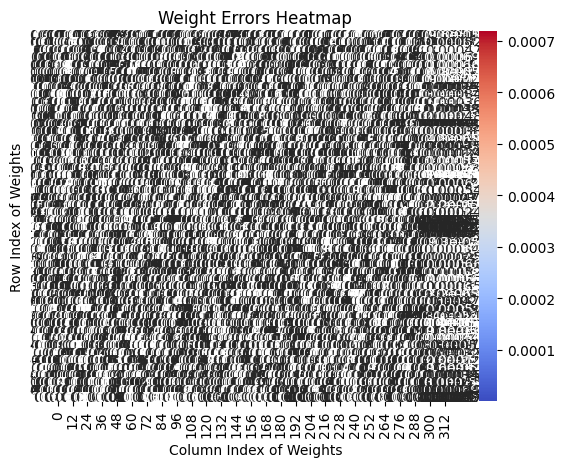
\includegraphics[width=\textwidth]{images/weightdist.png}
	\caption{Distribution of weights}
	\label{weightdist}
\end{figure}

As we can see from the heatmap, the weight error distribution is actually very random. This means that the quantization error is not concentrated on any particular weight. This is a good sign as it means that the quanization does not affect any particular types of features of weights and can be used for any kind of weights.
\cleardoublepage
\typeout{}
\chapter{PEMAN and CNN using random convolutions}

The one downside to using PEMAN and CNN is that the number of multiplication operations required, even for a single image is staggeringly high. For example, for a $256\times 256$ image, the number of multiplication operations required for a $5 \times 5$ kernel (with appropriate padding) comes to

\begin{equation*}
	256 \times 256 \times 5 \times 5 = 1638400
\end{equation*}

This is for a single image from a signle channel of a single layer. For a single layer with 10 channels, the number of multiplication operations required comes to

\begin{equation*}
	256 \times 256 \times 5 \times 5 \times 10 = 16384000
\end{equation*}

This is an absurdly large number and it is for an well known small dataset like MNIST. Surely, it is much larger for more complicated datasets. This is the reason why CNNs are so computationally expensive.

One possible way to reduce this proposed in this thesis. Although this idea is proposed, it is not explored very well and is not optimized, which is left to future works as it is out of the scope of this thesis.

To reduce the number of computations, the proposed idea is to take the total number of operations and take a fraction of it, say 90\%. Then, instead of performing the convolution operation on the entire image, the convolution operation is performed on random pixels of the image, instead of sliding over the image with a fixed stride. The pixels that were not chosen are given random values in the feature map. This is illustrated in the figure \ref{fig:randomScanning}.

\begin{figure}[h]
	\centering
	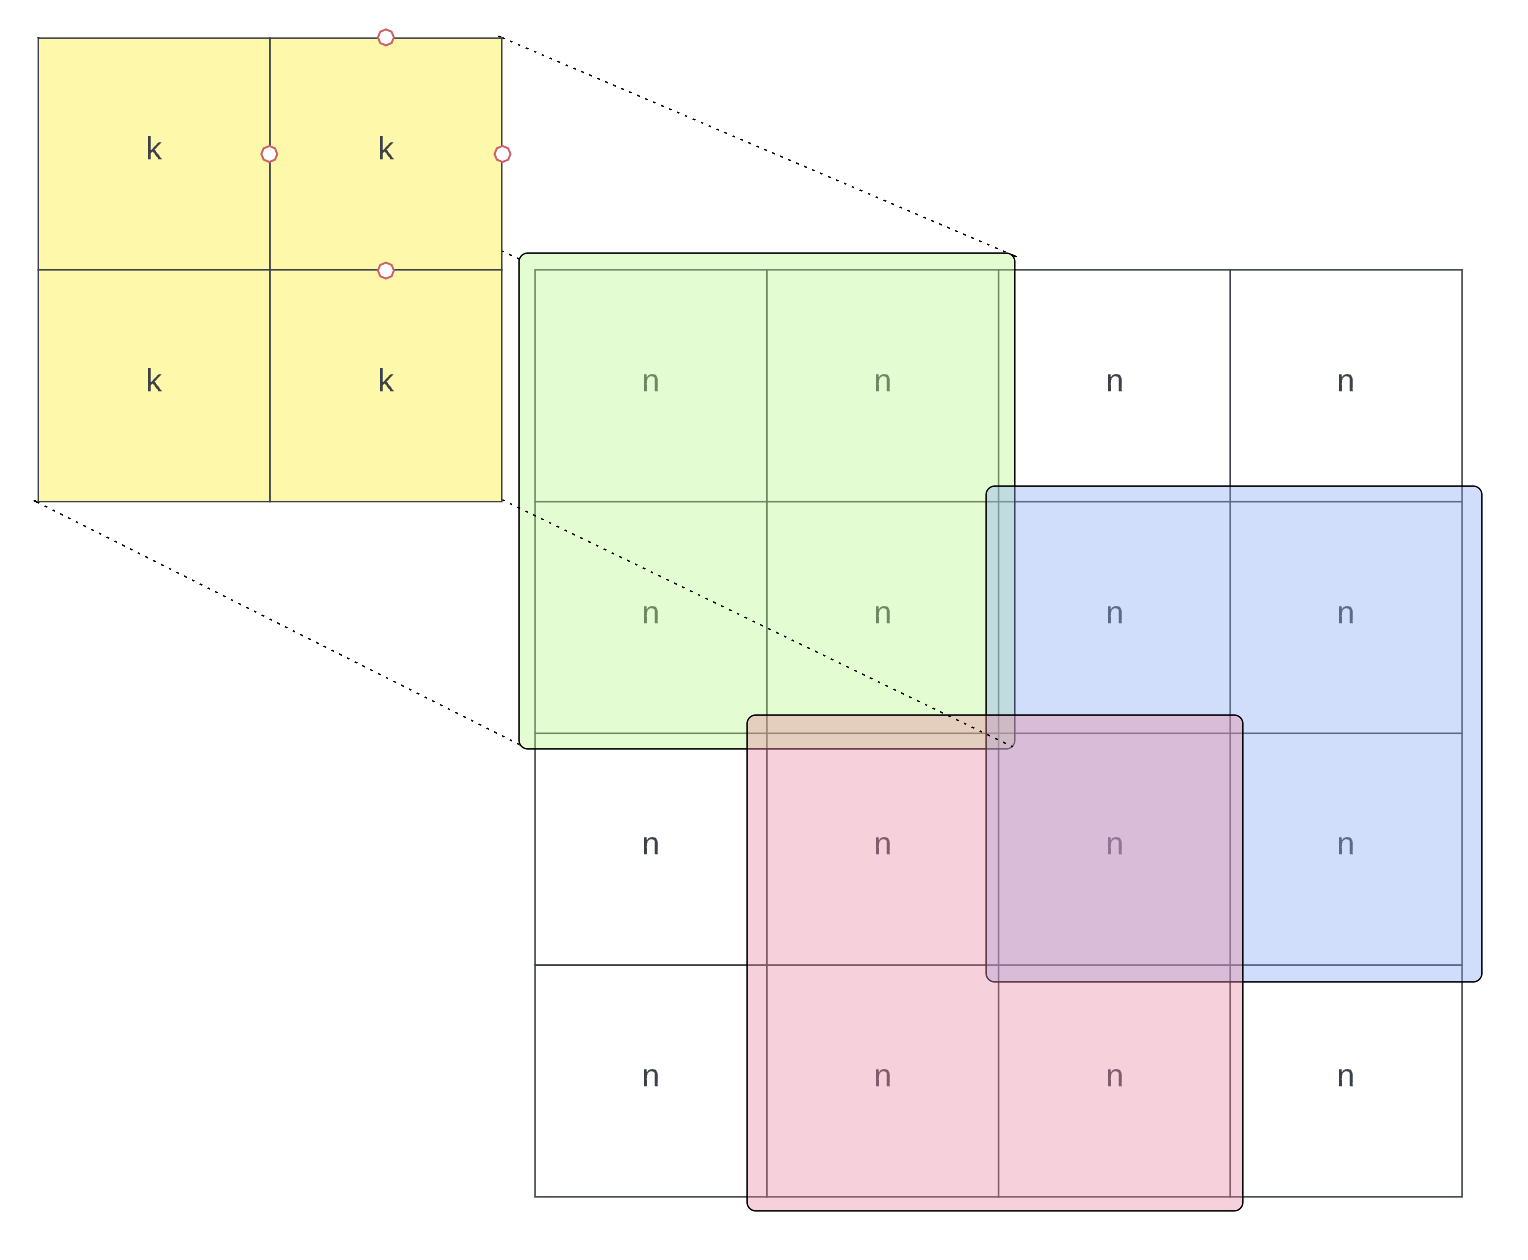
\includegraphics[width=0.8\textwidth]{images/randomScanning}
	\caption{Random scanning of the image}
	\label{fig:randomScanning}
\end{figure}

This type of convolution when used only during inference using PEMAN could drastically reduce the number of operations required and would thereby boost the speed of the structure. The tradeoff is that the accuracy of the model would be reduced.

After changing the exact same model from previous study to use random scanning during inference, the accuracy came out to be 18.78\%. This is significantly lower than previous models and is paractically not acceptable. Thus, this method needs to be explored further and researched as to which model and architecture would benefit this method the most.
\cleardoublepage
\typeout{}
\chapter{Conclusion and Future Work}

write results of your thesis and future work.




\typeout{}

\bibliographystyle{IEEEtran}
\bibliography{IEEEabrv,btp}
\end{document}
